\subsection{GUI}
\subsubsection{Overview}
The GUI is built with \texttt{pygame} for end-to-end interaction: input selection, manual play, AI solving, and result display. A modular screen/component design keeps rendering and gameplay logic maintainable.

\subsubsection{Screen Flow}
The interface follows a simple state flow:
\begin{itemize}
    \item \textbf{Menu}: Play, AI Solver, Exit.
    \item \textbf{Selection}: choose board size and input file.
    \item \textbf{Game}: manual play or AI visualization.
\end{itemize}

\begin{figure}[H]
    \centering
    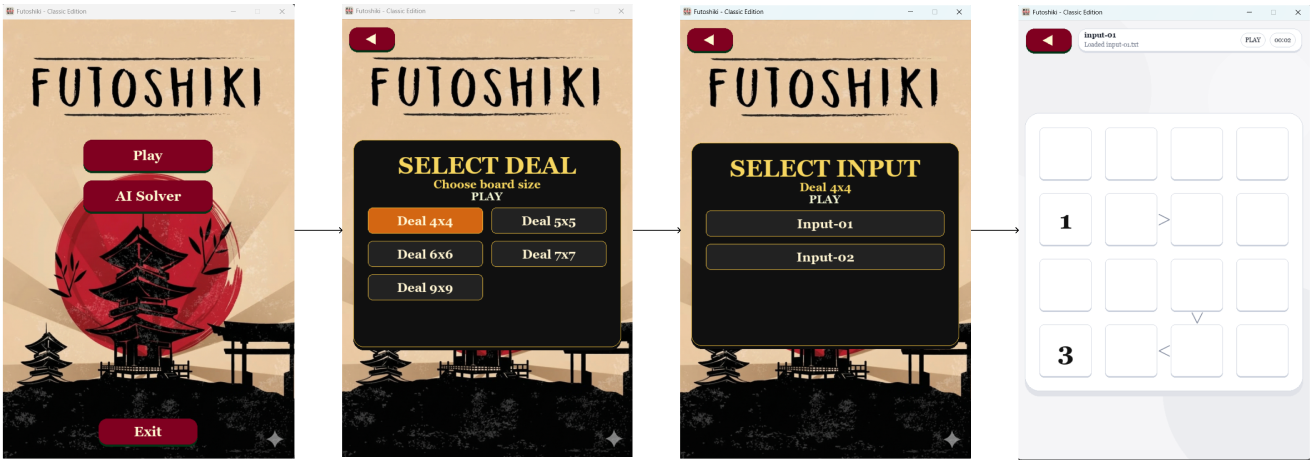
\includegraphics[width=0.9\linewidth]{image/gui_screen.png}
    \caption{GUI screen flow from menu to gameplay.}
    \label{fig:gui-screen-flow}
\end{figure}

\subsubsection{Gameplay Interface}
The gameplay screen renders the grid, keeps clue cells fixed, and validates moves in real time. Main controls:
\begin{itemize}
    \item click to select a cell;
    \item keys \(1\) to \(N\) to fill values;
    \item Backspace/Delete/0 to clear;
    \item timer display.
\end{itemize}
Inequality symbols are shown between cells, and completion is announced when all constraints are satisfied.

\begin{figure}[H]
    \centering
    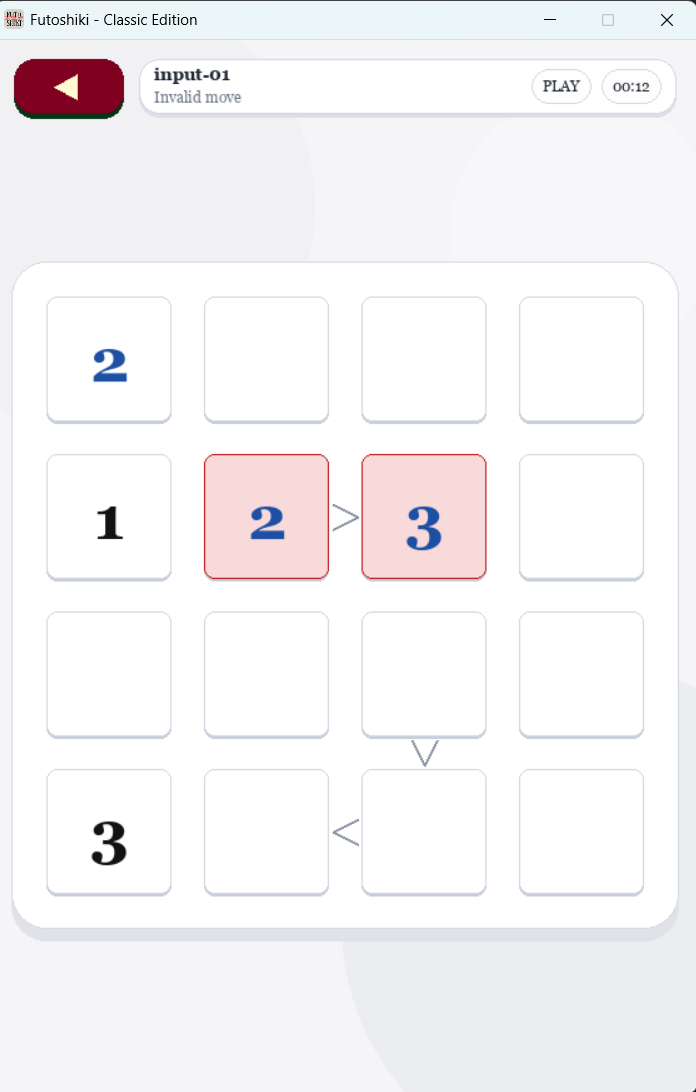
\includegraphics[width=0.9\linewidth]{image/gameplay.png}
    \caption{Main gameplay interface in manual mode.}
    \label{fig:gui-gameplay}
\end{figure}

\subsubsection{AI Solver Visualization}
AI visualization is handled by \texttt{AISolverManager} with a worker thread and step queue, so the UI remains responsive while solving. Solver steps are streamed incrementally to the board so users can observe the solving process.

Key behaviors:
\begin{itemize}
    \item highlight current solver actions;
    \item distinguish backtracking steps;
    \item allow skipping remaining animation;
    \item validate final state before showing solved status.
\end{itemize}

\begin{figure}[H]
    \centering
    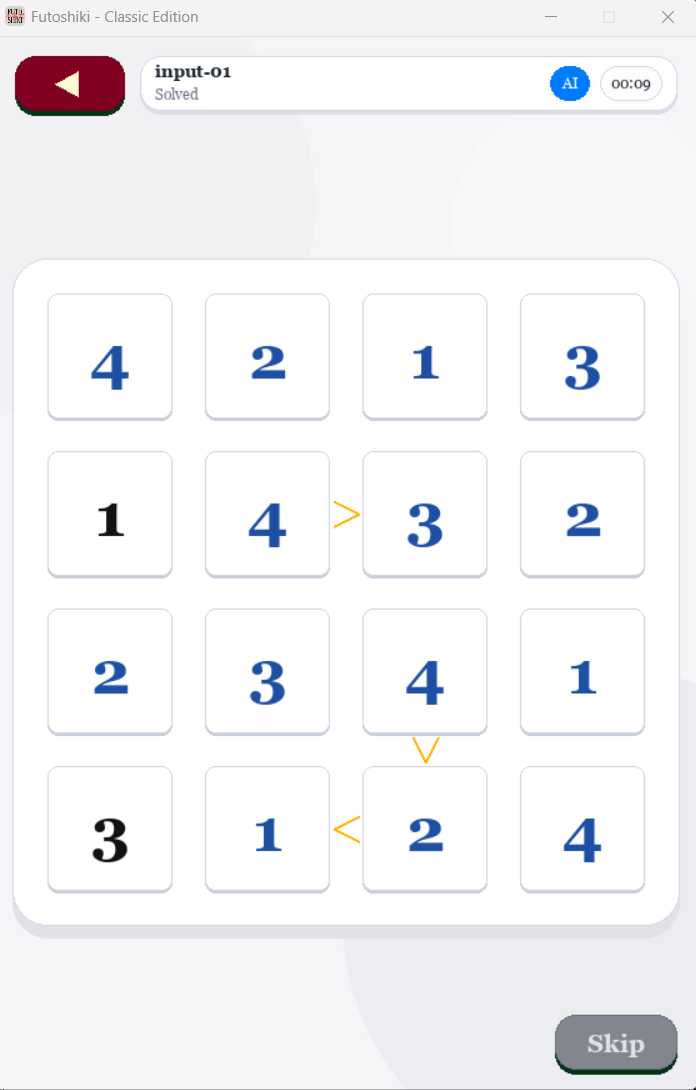
\includegraphics[width=0.9\linewidth]{image/ai_solver.png}
    \caption{Step-by-step AI solver visualization on the game screen.}
    \label{fig:gui-ai-animation}
\end{figure}

\subsubsection{Visual Design}
The visual style is simple and consistent to prioritize board readability and solver progress. Reusable UI components keep interactions uniform and implementation complexity low.

Overall, the GUI bridges puzzle data, user interaction, and solver execution in a practical way.
